\documentclass{article}
\usepackage{graphicx}
\graphicspath{ {../graphs/} }
\usepackage{geometry}
\geometry{a4paper, portrait, margin=1.0in}
\usepackage{booktabs}
\title{Computational Physics Project B1\\A Log Likelihood fit for extracting the $D^{0}$ lifetime} % Title

\author{Robert \textsc{Stein}} % Author name

\date{\today} % Date for the report

\begin{document}

\maketitle % Insert the title, author and date
\section{Abstract}
Finite Differential Methods (FDMs) are methods to solve 

\section{Aims and Implementation}
The basis for this analysis is a dataset containing many measurements with varying associated errors. A simple histogram shows the heavily-smeared raw distribution in Figure \ref{fig:decaytimes}. It arises from a convolution of the true exponential decay distribution and Gaussian smearing arising from measurement uncertainty. 
\begin{figure}
\begin{center}
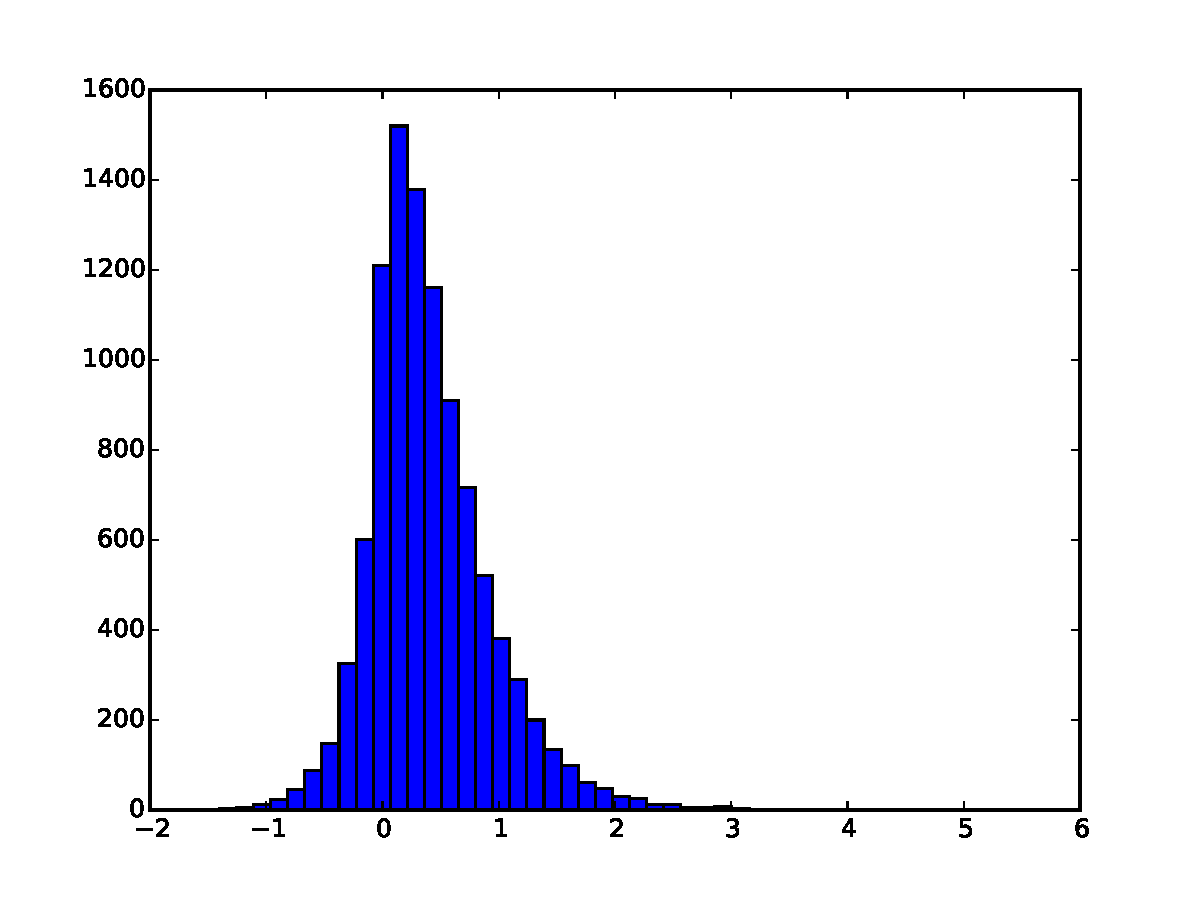
\includegraphics[height=0.25\textheight]{decaytimes}
\caption{The reconstructed decay times of $D^{0}$ mesons.}
\label{fig:decaytimes}
\end{center}
\end{figure}

From the data, we wish to obtain the most probable value for the decay constant $\tau$. We choose a $\tau$ which maximises the likelihood of obtaining the results, and thus minimises the Negative Log Likelihood (NLL) of the dataset. A convenient consequence of considering NLL rather than Likelihood directly is that the NLL of a dataset is simply a sum of the component from each measurement, rather than a product of many values.

The experimental value of $\tau$ can be obtained through a simple 1D minimisation of the function $NLL(\tau)$, using a parabolic minimiser. A parabolic minimiser begins with three starting values $x_{0}$, $x_{1}$ and $x_{2}$. With $y_{i} = f(x_{i})$ for a function f, we can calculate the values $x_{3}$ and $y_{3}$.

\[x_{3} = \frac{1}{2} \frac{(x_{2}^{2}-x_{1}^{2})y_{0} + (x_{0}^{2}-x_{2}^{2})y_{1} + (x_{1}^{2}-x_{0}^{2})y_{2}}{(x_{2}-x_{1})y_{0} + (x_{0}-x_{2})y_{1} + (x_{1}-x_{0})y_{2}}\] 

The parameter $x_{i}$ with the largest corresponding $y_{i}$ value is eliminated, and the remaining three values are relabelled. The process is repeated until convergence on a minimum occurs. 

Alternatively, the small number of background events $N_{bkg}$ can also be considered. In general, we define $a = \frac{N_{sig}}{N_{bkg}+N_{sig}}$. We can consider the total likelihood of each event as the weighted sum of probabilities: 

\[ Likelihood = a P_{sig}(t \mid \tau, \sigma)  + (1-a) P_{bkg}(t \mid \tau, \sigma) \]

The NLL is again found for the purposes of minimisation. A Quasi-Newton minimiser was implemented for 2D minimisation, following an iterative process, with $G_{0}$ being the 2D identity matrix.

\[ \mathbf{x_{n+1}} = \mathbf{x_{n}} - \alpha G_{n} \cdot \nabla f(\mathbf{x_{n}}) \]

\[ G_{n+1} = G_{n} + \frac{(\mathbf{\delta_{n}} \otimes \mathbf{\delta_{n}})}{\mathbf{\gamma_{n}} \cdot \mathbf{\delta_{n}}} - \frac{G_{n} \cdot (\mathbf{\delta_{n}} \otimes \mathbf{\delta_{n}}) \cdot G_{n}}{\mathbf{\gamma_{n}} \cdot G_{n} \cdot \mathbf{\gamma_{n}}}\]

\[ \mathbf{\delta_{n}} \equiv \mathbf{x_{n+1}} - \mathbf{x_{n}} \]

\[ \mathbf{\gamma_{n}} \equiv \nabla f(\mathbf{x_{n+1}}) - \nabla f(\mathbf{x_{n}}) \]

In both cases, a definition of convergence is required to terminate the iterative process. in terms of change in NLL rather than parameter space distance. 

We find a minimum $\mathbf{x_{min}} = \sum_{i} x_{i}$ for dimensions i. From the definition of  

\section{Code Validation}
Other function. cosh(x)

An effective way to validate the minimisation process is to produce a graph of the function NLL. This is done in Figures \ref{fig:nll1d} and \ref{fig:nll2d} for the 1D and 2D minimsations respectively. In both cases, a broad minimisation region is clear, providing a useful sanity check on minimiser results. However, the production of such graphs is extremely resource-intensive. The iterative process required to obtain precise results in this manner is thus inefficient, limiting the effectiveness of such validation to perhaps one order of magnitude.

\begin{figure}
\begin{center}
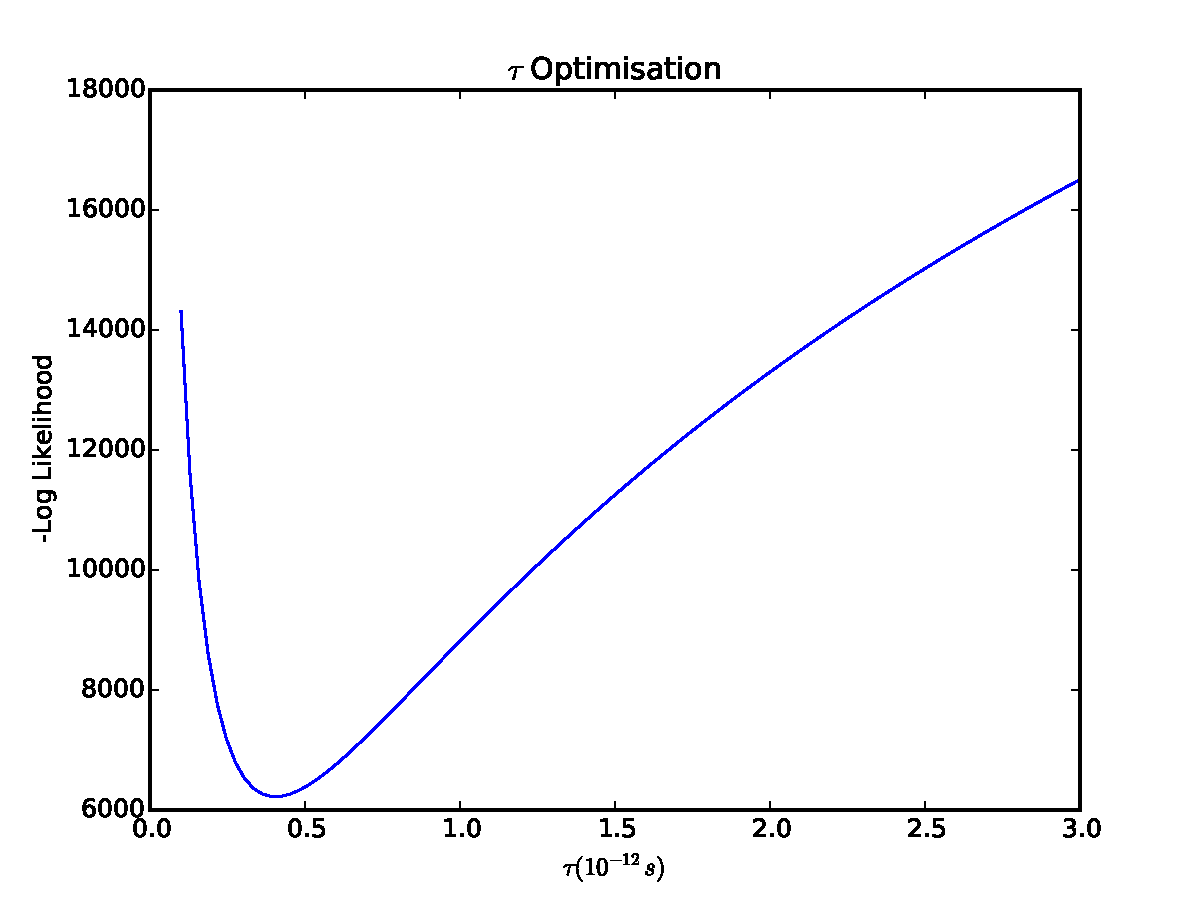
\includegraphics[height=0.3\textheight]{nll}
\caption{The function $NLL(\tau)$ against $\tau$. The minimum clearly lies in the region of $0.4 < \tau < 0.5$.}
\label{fig:nll1d}
\end{center}
\end{figure}

\begin{figure}
\begin{center}
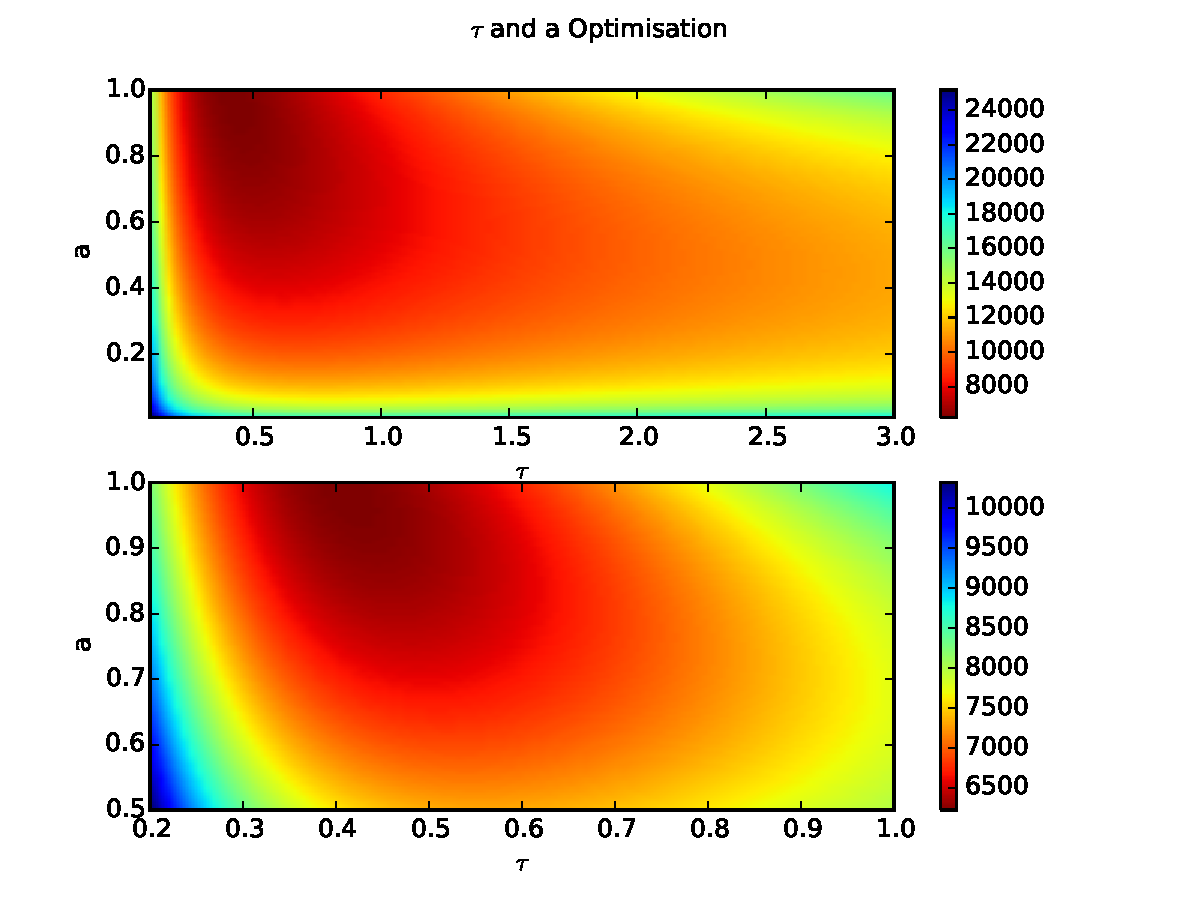
\includegraphics[height=0.3\textheight]{nll2d}
\caption{Graphs of a against $\tau$, with the colour scale representing function $NLL(\tau, a)$. The above graph covers the entire minimisation region, showing the minimum lying in the region $0.2 < \tau < 1.0$ and $0.5 < a < 1.0$. The lower graph focuses exclusively on this low-NLL region to provide higher contrast. With the new colour scale, it is clear that $0.3 < \tau < 0.6$ and $0.7 < a < 1.0$. We expect the minimisation solution to lie in this region. The path of the minimisation is shown in white, beginning at the cross and ending at the star.}
\label{fig:nll2d}
\end{center}
\end{figure}

\section{Results}

etc.

\begin{figure}
\begin{center}
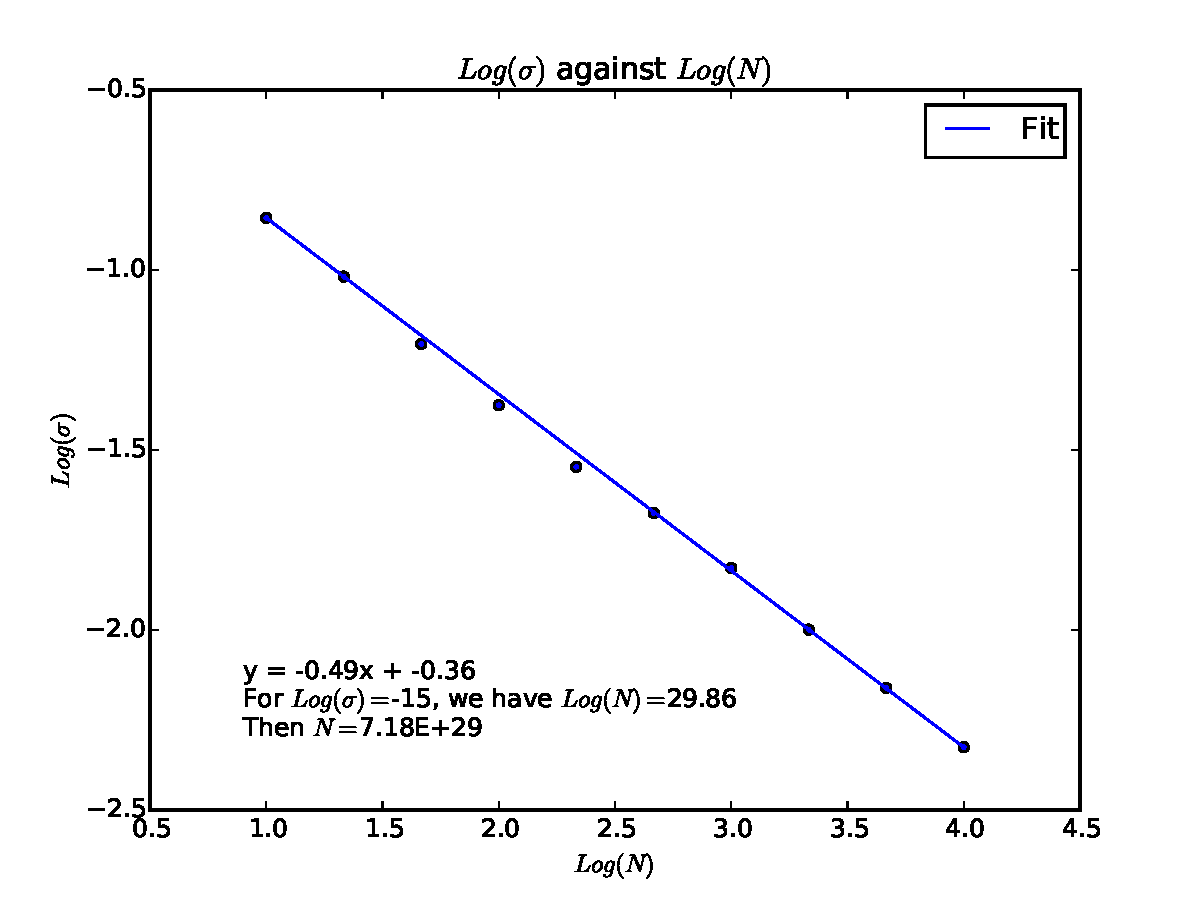
\includegraphics[height=0.3\textheight]{nsigma}
\caption{A graph of $\log(\sigma)$ against $\log(n)$ }
\label{fig:nsigma}
\end{center}
\end{figure}

\section{discussion}

moar

\section{Conclusion}
end

\end{document}